\documentclass[titlepage,a4paper,12pt]{report}
\usepackage{amssymb,amsfonts,amsmath}
\usepackage{tikz}
\usetikzlibrary{arrows}
\newcommand\Interval[4]{%
  \begin{tikzpicture}[text height=1ex]%
    \draw[<-] (0,0) -- (1,0);
    \draw[{#3-#4}] (1,0) node[label=below:{#1}] {} -- (2,0) node[label=below:{#2}] {};
    \draw[->] (2,0) -- (3,0);
  \end{tikzpicture}
}
%\usepackage{fullpage}
\usepackage{graphicx}
%\usepackage[cc]{titlepic}
\usepackage{amsthm}
\newtheorem{definition}{Definition}[section]
\newtheorem{example}{Example}[section]
\newtheorem{theorem}{Theorem}[section]
\newtheorem{exercise}{Exercise}[section]
\newtheorem{corollary}{Corollary}[section]
\newtheorem{proposition}{Proposition}[section]
\pdfpagewidth 8.5in
\pdfpageheight 11in
\setlength\topmargin{-0.5in}
\setlength\headheight{0in}
\setlength\headsep{0in}
\setlength\textheight{9.5in}
\setlength\textwidth{7.0in}
\setlength\oddsidemargin{-0.5in}
\setlength\evensidemargin{1.0in}
\setlength\parindent{0.25in}
\setlength\parskip{0.25in}
%\begin{titlepage}
%\usepackage{titlepic}
%\titlepic{
\includegraphics[width=0.2\textwidth]{uz1.png}}
%
%\title{\textbf{HMTH111 Calculus 2}}
%\author{Nhawu. G\\
%		Department of Mathematics\\
%		University of Zimbabwe, ZIM}
%
%\end{titlepage}

\begin{document}
\begin{titlepage}
 
\begin{center}
 
 
% Upper part of the page

\includegraphics[width=0.15\textwidth]{uz1.png}\\[1cm]
 
\textsc{\LARGE University of Zimbabwe}\\[1.5cm]
 
\textsc{\Large HMTH101 CALCULUS 1}\\[0.5cm]
 
 
% Title

{ \huge \bfseries Calculus of Single Variables}\\[0.4cm]
 

 
% Author and supervisor
\begin{minipage}{0.4\textwidth}
\begin{center} \large
\emph{Author:}\\
G. \textsc{Nhawu}
\end{center}
\end{minipage}
\begin{minipage}{0.4\textwidth}
\begin{flushright} \large
\emph{Department:} \\
\textsc{Mathematics}
\end{flushright}
\end{minipage}

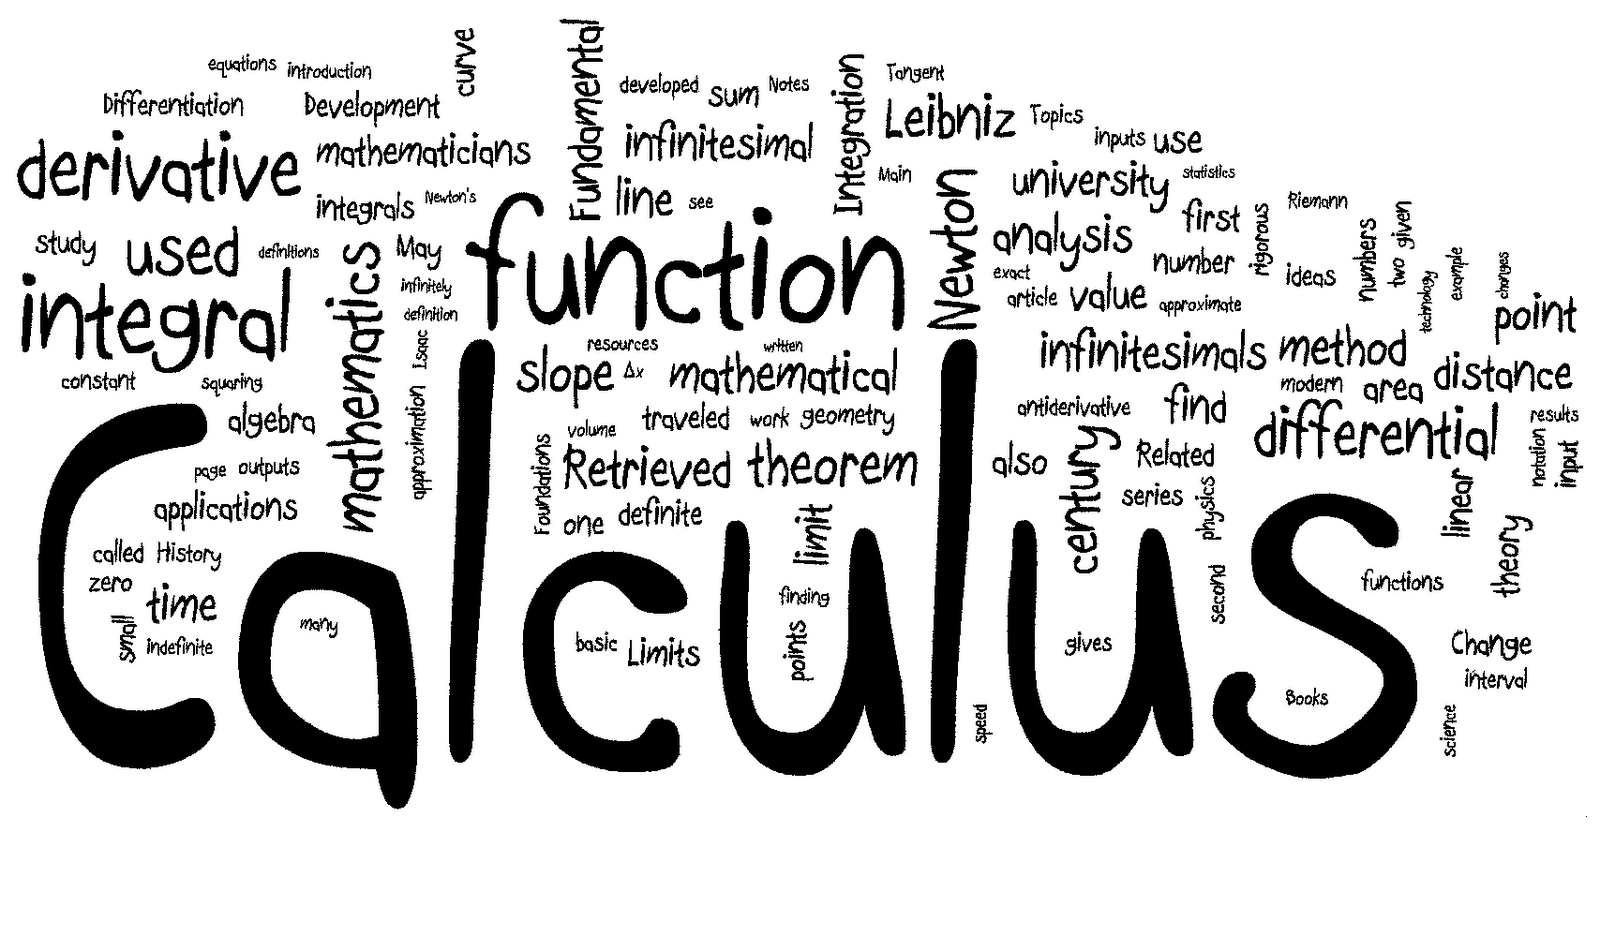
\includegraphics[width=0.98\textwidth]{calculus2.png}\\[1cm]
 \vfill
 
 
% Bottom of the page
{\large \today}
 
\end{center}
 
\end{titlepage}

\chapter{Functions}
\begin{center}
	\small{\parbox{18cm}{
		\begin{raggedright}
		{\small
		\textit{We know that God exists because Mathematics is consistent and we know that the devil exists because we cannot prove the consistency.}
 }
 
				\vspace{.5cm}\hfill{---Andre Weil}
		\end{raggedright}
	}
} 
\end{center}
\section{What is a Function?}
\noindent A function is a \textit{rule} or a \textit{correspondence}, relating two sets in such a manner that each element in the first set corresponds to one and only one element in the second set. What do we mean when we say $\boxed{y ~~is~~ a ~~function~~ of~~ x?}$ Symbolically, we write $y=f(x)$, where 
\begin{enumerate}
\item $x$ is the \textit{independent variable}. (input value of $f$)
\item $y$ is the \textit{dependent variable}. (output value of $f$ at $x$)
\item $f$ is a \textit{function}. (rule that assigns $x$ to $y$)
\end{enumerate}
\begin{definition}
A function $f$ from a set $X$ to a set $Y$ is a rule that assigns to each element $x$ in $X$ a unique element $y$ in $Y$.
\end{definition}
The set $X$ is called the \textbf{domain} of $f$ and the set of corresponding elements $y$ in $Y$ is called the \textbf{range} of $f$ where sets $X$ and $Y$ consists of real numbers. We write $f :X\to Y$.

\noindent \textbf{Examples:} Stock market index depending on time, volume of sphere depending on radius, circle of a given radius has only one area.

\noindent Let $f$ be a function. The number $y$ in the range that corresponds to a selected number $x$ in the domain is said to be the value of the function at $x$, or \textbf{image} of $x$, written $f(x)$, so $y=f(x)$.

\noindent \textbf{Examples:} $f(x)=3x^4+2$, $g(t)=4-t^2$, $h(s)=2s^2+7$.

\noindent The \textbf{domain} of a function $f$ is the largest set of real numbers for which the rule makes sense.
\begin{center}
 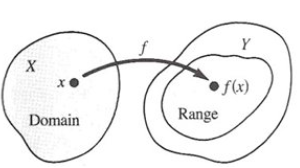
\includegraphics[width=0.4\textwidth]{function1.png}\\[1cm]
  \end{center}
 \textbf{Example:} Let $f(x)=\dfrac{1}{x}$, we cannot compute $f(0)$, since $\dfrac{1}{0}$ is not defined. Then the domain of $f(x)=\dfrac{1}{x}$ is the set of all real numbers except $0$.

\begin{table}[h]
\centering
\begin{tabular}{|l|c|c|}
\hline
\textbf{Function} & \textbf{Domain} $x\in X$ & \textbf{Range} $y\in Y$\\
\hline
$y=x^2$ & $(-\infty , \infty)$ & $[0,\infty)$ \\
$y=\dfrac{1}{x}$ & $(-\infty , 0)\cup (0, \infty)$ & $(-\infty , 0)\cup (0, \infty)$\\
$y=\sqrt{x}$ & $[0,\infty )$ &$[0,\infty )$\\
 $y=\sqrt{1-x^2}$ & $[-1,1]$ & $[0,1]$\\
\hline
\end{tabular}
\caption{Examples of functions}
\label{tab:template}
\end{table}

\noindent \textbf{You Try It:} Let 
\begin{equation*}
g(x)=\dfrac{x}{x^2+4x+3}.
\end{equation*}
What is the domain and range of this function?
\section{Graphs of Functions}
It is useful to draw pictures which represent functions. These pictures, or \textit{graphs}, are a device for helping us to think about functions. We graph functions in the $x-y$ pane. The elements of the domain of the function are thought of as points of the $x-$axis. The values of a function are measured on the $y-$axis.The graph of $f$ associates to $x$ a unique $y$ value that the function $f$ assigns to $x$. 
The \textbf{graph} of a function $f$ is the set of points $\{(x,y)| y=f(x) \quad \hbox{in the domain of $f$}\}$ in the Cartesian plane.

\noindent As a consequence, a function is characterised geometrically by the fact that any vertical line intersecting its graph does so in \textit{exactly one point}.
\begin{center}
 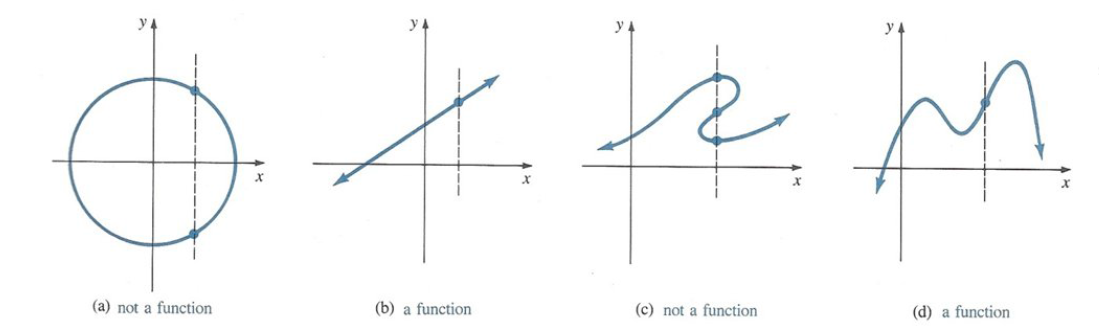
\includegraphics[width=0.89\textwidth]{2.png}\\[1cm]
  \end{center}

\section{Bounded Functions}
If there is a constant $M$ such that $f(x)\leq M$ for all $x$ in the interval (or other set of numbers), we say that $f$ is \textit{bounded above} in the interval (or the set) and call $M$ an \textit{upper bound} of the function. If a constant $m$ exists such that $f(x)\geq m$ for all $x$ in an interval, we sat that $f(x)$ is \textit{bounded below} in the interval and call $m$ a \textit{lower bound}. If $m\leq f(x)\leq M$ in an interval, we call $f(x)$ \textit{bounded}.

\noindent \textbf{Examples:} $f(x)=x+3$ is bounded in $-1\leq x\leq 1$. An upper bound is $4$ (or any number grater than $4$). A lower bound is $2$ (or any number less than $2$).  
\section{Types of Functions}
\subsection{Elementary Functions}
\subsubsection{Polynomial Function}
Have the form $f(x)=a_0x^n+a_1x^{n-1}+\cdots + a_{n-1}x+a_n$ where $a_0, a_1, \dots , a_n$ are constants and $n$ is a positive integer called the degree of the polynomial provided $a_0\neq 0$. 

\noindent \textbf{Examples:} $x^5+10x^3-2x+1$ is a polynomial of degree $5$.
\subsubsection{Rational Functions}
A function $f(x)=\dfrac{P(x)}{Q(x)}$ where $P(x)$ and $Q(x)$ are polynomial functions.

\noindent \textbf{Example:} $f(x)=\dfrac{x^3+x+5}{x^2-3x-4}$ is a rational function. Since $(x+1)(x-4)$ and $(x+1)(x-4)=0$ for $x=-1$ and $x=4$, the domain of $f$ is the set of all real numbers except $-1$ and $4$.  
\subsubsection{Power Function}
$f(x)=kx^n$, $n$ a real number and $k$ a constant. 
\begin{center}
 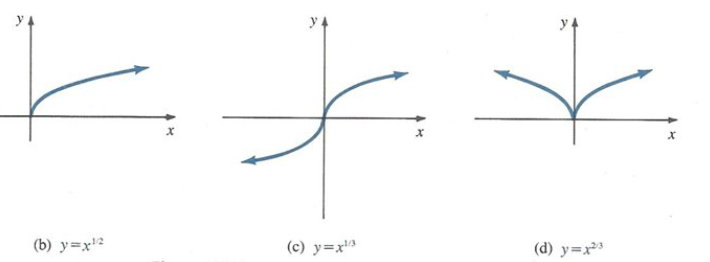
\includegraphics[width=0.6\textwidth]{power.png}\\[1cm]
  \end{center}
\noindent \textbf{Examples:} $y=\dfrac{1}{x}$, $y=x^{\frac{1}{2}}$, $y=x^{\frac{2}{3}}$.
\subsubsection{Piecewise Defined Functions}
A function need not be defined by a single formula. A piecewise defined function is a function described by using \textit{different formula on different parts of its domain}.

\noindent \textbf{Examples:} (a)\,  $f(x) = \left\{ 
\begin{array}{l l}
  -1, & \quad  x<0 \\
 0, & \quad x=0\\
 x+2, & \quad x>0\\ \end{array} \right. $ \quad (b)\, $f(x) = \left\{ 
\begin{array}{l l}
  -x, & \quad  x< 0 \\
 x^2, & \quad 0\leq x\leq 1\\
 1, & \quad x>1.\\ \end{array} \right. $
 \begin{center}
 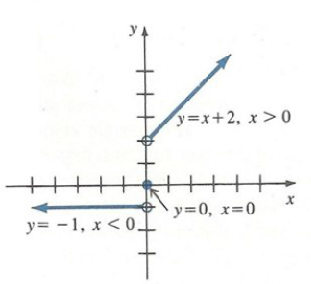
\includegraphics[width=0.6\textwidth]{piece.png}\\[1cm]
  \end{center}
 \subsubsection*{Transcendental  Functions}
 The following are sometimes called \textit{elementary transcendental functions}.
 \begin{enumerate}
 \item  Exponential function, $f(x)=a^x, a\neq 0,1$.
 \item Logarithmic  function, $f(x)=\log _a x, a\neq 0,1$.
 \item Trigonometric functions (also called circular functions because of their geometric interpretation with respect to the unit circle), e.g., $\sin x, \cos x, \tan x =\dfrac{\sin x}{\cos x}, \csc x, \cot x, \sec x$.
 \item Inverse trigonometric functions, e.g., $y=\sin ^{-1} x, y=\cos ^{-1} x$.
 \item Hyperbolic Functions, e.g., $\sinh x, \cosh x, \tanh x, \coth x$.
  \end{enumerate}
  \subsubsection{Even and Odd Functions}
  Let $f(x)$ be a \textit{real-valued} function of a real variable. Then $f$ is \textit{even} if $f(x)=f(-x)$. (Symmetric with respect to the $y-$axis)
  
\noindent \textbf{Examples:} $|x|, x^2, x^4, \cos x, \cosh x$.

\noindent Let $f(x)$ be a real-valued function of a real variable. Then $f$ is \textit{odd} if $-f(x)=f(-x)$ or \\$f(x)+f(-x)=0$. (Symmetric with respect to the origin)

\noindent \textbf{Examples:} $x, x^3, \sin x, \sinh x$.

\noindent \textbf{Example:} Determine whether the following function is odd or even $f(x)=\dfrac{3x}{x^2+1}$.

\noindent \textbf{Solution:} \begin{equation*}
f(-x)=\dfrac{3(-x)}{(-x)^2+1}=-\dfrac{3x}{x^2+1}=-f(x).
\end{equation*}
The function is odd.
\section{Combining Functions}
A function $f$ can be combined with another function $g$ by means of arithmetic operations to form other functions, the \textbf{sum} $f+g$, \textbf{difference} $f-g$, \textbf{product} $fg$ and \textbf{quotient} $\dfrac{f}{g}$ are defined as : Let $f$ and $g$ denote functions, then 
\begin{enumerate}
\item \underline{Sum} : $(f+g)(x)=f(x)+g(x)$.
\item \underline{Difference} : $(f-g)(x)=f(x)-g(x)$.
\item \underline{Product} : $(fg)(x)=f(x)g(x)$.
\item \underline{Quotient} : $\left(\dfrac{f}{g}\right )(x)=\dfrac{f(x)}{g(x)}$.
\end{enumerate}
\textbf{Example:} If $f(x)=2x^2-5$ and $g(x)=3x+4$. Find $f+g, f-g, fg, \dfrac{f}{g}$.

\noindent \textbf{Solution:} \begin{eqnarray*}
(f+g)(x) &=& (2x^2-5)+(3x+4)= 2x^2+3x-1.\\
(f-g)(x)&=& (2x^2-5)-(3x+4)= 2x^2-3x-9.\\
(fg)(x)&=&(2x^2-5)(3x+4) = 6x^3+8x^2-15x-20\\
\left(\dfrac{f}{g}\right)(x)&=& \dfrac{2x^2-5}{3x+4}.\\
\end{eqnarray*}
\section{Composition of Functions}
Let $f$ and $g$ denote functions. The \textbf{composition } of $f$ and $g$, written $f\circ g$ is the function $(f\circ g)(x)=f(g(x))$ and the composition of $g$ and $f$, written $g\circ f$, is the function $(g\circ f)(x)=g(f(x))$.

\noindent \textbf{Example:} If $f(x)=x^2$ and $g(x)=x^2+1$, find $f\circ g$ and $g \circ f$.

\noindent \textbf{Solution:} \begin{equation*}
(f\circ g)(x)=f(g(x))=f(x^2+1)=(x^2+1)^2=x^4+2x^2+1.
\end{equation*}
and \begin{equation*}
(g\circ f)(x)=g(f(x))=g(x^2)=(x^2)^2+1=x^4+1.
\end{equation*}
In general, $f\circ g \neq g\circ f$.
\section{Bijection, Injection and Surjection}
Classes of functions may be distinguished by the manner in which arguments and images are related or \textit{mapped} to each other.

\noindent A function $f:X\to Y$ is \textbf{injective (one-to-one, $1-1$)} if every element of the range corresponds to exactly one element in its domain $X$.

\noindent For all $x,y\in X$, $f(x)=f(y)\Longrightarrow x=y$ or equivalently

\noindent For all $x,y\in X$, $x\neq y\Longrightarrow f(x)\neq f(y)$.  An injective function is an \textbf{injection}.

\begin{center}
 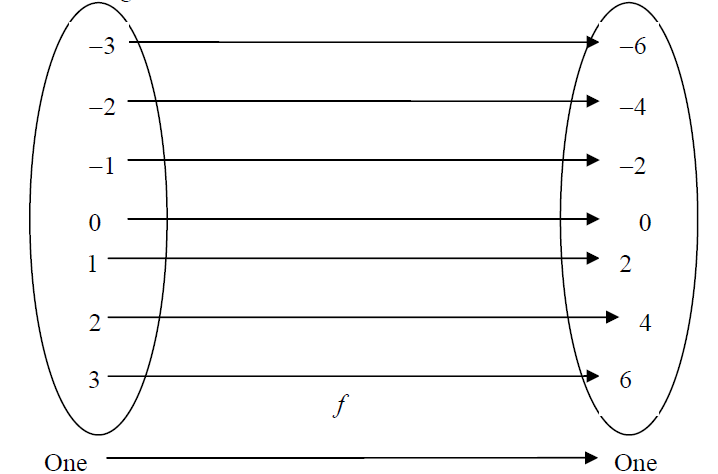
\includegraphics[width=0.6\textwidth]{one.png}\\[1cm]
  \end{center}
\noindent \textbf{Example:} Show that the functions $f(x)=2x+3$ and $g(x)=x^3-2$ are injective.

\noindent \textbf{Solution:} Need to show that $f(x)=f(y)\Longrightarrow x=y$.
\begin{eqnarray*}
2x+3 &=& 2y+3 \\
2x &=& 2y \Longrightarrow x =y.\\
\end{eqnarray*}
Hence $f(x)=2x+3$ is injective.

\noindent Need to show that $g(x)=g(y)\Longrightarrow x=y$.
\begin{eqnarray*}
x^3-2 &=& y^3-2 \\
x^3 &=& y^3 \quad  \hbox{taking cube roots}\\
x &=& y.
\end{eqnarray*}
Hence $g(x)=x^3-2$ is injective.

\noindent A function $f:X\to Y$ is called \textbf{onto} if for all $y$ in $Y$ there is an $x$ in $X$ such that $f(x)=y$. All elements in $Y$ are used. Such functions are referred to as \textbf{surjective}.
\begin{center}
 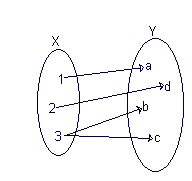
\includegraphics[width=0.2\textwidth]{save.png}\\[1cm]
  \end{center}
\noindent \textbf{Example:} Show that $f(x)=3x-5$ is onto.

\noindent \textbf{Solution:} For \textit{onto} $f(x)=y$, i.e., $3x-5=y$. Solve for $x$, $\Longrightarrow x=\dfrac{y+5}{3}$.\\ So $f\left (\dfrac{y+5}{3}\right)=3\left(\dfrac{y+5}{3} \right)-5=y$. Therefore $f$ is onto.

\noindent  Let $X$ and $Y$ be sets. A function $f:X\to Y$ that is one-to-one and onto is called a \textit{bijection} or \textit{bijective function from $X$ to $Y$}. If $f$ is both one-to-one and onto, then we call $f$ a $1-1$ correspondence.

\noindent \textbf{Inverse of a Function.} Suppose $f$ is a $1-1$ function that has domain $X$ and range $Y$. Since every element $y\in Y$ corresponds with precisely one element $x$ of $X$, the function $f$ must actually determine a \textit{reverse} function $g$ whose domain is $Y$ and range is $X$, where $f$ and $g$ must satisfy $f(x)=y$ and $g(y)=x$. The function $g$ is given the formal name \textit{inverse} of $f$ and usually written $f^{-1}$ and read $f$ inverse. Not all functions have inverses, those that do are called \textit{invertible functions}.
\begin{center}
 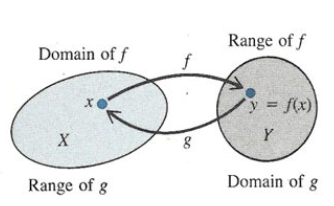
\includegraphics[width=0.6\textwidth]{inverse.png}\\[1cm]
  \end{center}
\noindent \textbf{Example:} Find the inverse of the function $f(x)=(2x+8)^3$.

\noindent \textbf{Solution:} We must solve the equation $y=(2x+8)^3$ for $x$.
\begin{eqnarray*}
y &=& (2x+8)^3\\
\sqrt[3]{y} &=& 2x+8 \\
\sqrt[3]{y}-8 &=& 2x \\
x &=& \dfrac{\sqrt[3]{y}-8}{2}.
\end{eqnarray*}
Hence the inverse function $f^{-1}$ is given by $f^{-1}(x)= \dfrac{\sqrt[3]{x}-8}{2}$.

\noindent A $1-1$ function $f$ can have only one inverse, i.e., $f^{-1}$ is unique. A function $f:X\to Y$ is \textbf{invertible} if and only if $f$ is one-to-one and maps $X$ onto $Y$.

\section{Operations on Functions}
\subsubsection{Equality of Functions}
Equality of functions does not mean the same as equality of two numbers (numbers have a fixed value but values of functions vary). Each function is a relationship between $x$ and $y$, the two relationships are the same if for every value of $x$ we get the same value of $y$.

\noindent \textbf{Example:} The functions $(x-1)(x+2)$ and $x^2+x-2$ are equal.

\noindent \textbf{Example:} Equal functions for positive values of $x$,
\begin{equation*}
|x| =\sqrt{x^2}.
\end{equation*}
\subsubsection{Identity Function}
Generally, an identity function is one which does not change the domain values at all. Its the function $f(x)=x$. Denoted by $I_X$.
\begin{center}
 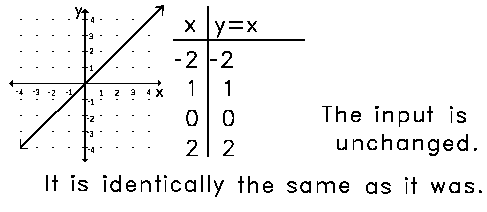
\includegraphics[width=0.6\textwidth]{identity.png}\\[1cm]
  \end{center}
\subsubsection{Monotonic Functions}
A function is called \textit{monotonic increasing} in an interval, if for any two points $x_1$ and $x_2$ in the interval such that if $x_1<x_2, \, f(x_1)\leq f(x_2)$. If $f(x_1)<f(x_2)$ the function is called \textit{strictly increasing}.

\noindent \textbf{Similarly}, if $f(x_1)\geq f(x_2)$ whenever $x_1< x_2$, then $f(x)$ is \textit{monotonic decreasing},  while if \\$f(x_1)>f(x_2)$ it is \textit{strictly decreasing}.
\section{Tutorial Questions}
\begin{enumerate}
\item Find the domain of each of the following functions.\\
(i)\, $-\sqrt{9-x^2}$  \quad (ii)\, $\dfrac{1}{\sqrt{1-x}}$ \quad (iii)\, $\dfrac{1}{2x+3}$ \quad (iv)\, $\sqrt{(3-x)(2x+4)}$ \quad (v)\, $\dfrac{x-2}{x^2-4}$ \\ (vi)\, $\ln (x^3-3x^2-4x+12)$ \quad (vii)\, $\dfrac{x^3-8}{x^2-4}$ \quad (viii)\, $\sqrt{\sin 5x}$ \quad  (ix)\, $\ln (2x^2-5x-12)$ \\(x)\, $\dfrac{1}{\sqrt{9-x^2}}$ \quad (xi)\, $\sqrt{x^2-4}$ \quad (xii)\, $x^2+4$ \quad (xiii)\, $\sqrt{\dfrac{x}{2-x}}$.
\item If $f(x)=\dfrac{x-1}{x+1}$, find (i)\, $f(0)$ \quad (ii)\, $f(1)$ \quad (iii)\, $f(-2)$. Show that $f\left(\dfrac{1}{x}\right)=-f(x)$ and $f\left(-\dfrac{1}{x}\right)=-\dfrac{1}{f(x)}$.
\item If $f(x)=\dfrac{1}{x}$, show that $f(a)-f(b)=f\left(\dfrac{ab}{b-a} \right)$.
\item If $f(x)=x^2-x$, show that $f(x+1)=f(-x)$.
\item If $y=f(x)=\dfrac{5x+3}{4x-5}$, show that $x=f(y)$.
\item Determine whether or not each of the following correspondences is a function.\\
(i)\, $x^2+y=1$ \quad (ii)\, $x^2y^2=5$ \quad (iii)\, $x^2y=4$ \quad (iv)\, $\{(1,5), (2,5), (5,1)\}$.
\item For each of the following pairs of functions, calculate $f\circ g$ and $g\circ f$.
\begin{itemize}
\item[(i)] $f(x)=\sin (x+3x^2)$ and $g(x)=\cos (x^2-x)$.
\item[(ii)] $f(x)=e^{x^2}$ and $g(x)=e^{-x^2}$.
\item[(iii)] $f(x)=x(x+1)(x+2)$ and $g(x)=(2x-3)(x+4)$.
\end{itemize}
\item Determine whether each of the pairs of the following functions are equal and if they are not equal, give where they are equal.\\
(i)\, $f(x)=\sqrt{x^2}, \quad g(x)=(\sqrt{x})^2$ \quad (ii)\, $f(x)=x^2, \quad g(x)=x|x|$.
\item Show that if $ad-bc\neq 0$, then the function $f(x)=\dfrac{ax+b}{cx+d}$ is one-to-one and find its inverse, stating the domains of both the function and its inverse. What happens if $ad-bc=0$?
\item Show that these functions are a one-to-one correspondence. Find their inverses.\\
(i)\, $f(x)=2x+3$ \quad (ii)\, $g(x)=x^3-2$ \quad (iii)\, $h(x)=(x-2)^2$ \quad (iv)\, $k(x)=\sqrt[3]{x}+7$.
\item Show that the function $f(x)=\ln (x+\sqrt{x^2+1})$ is an odd function and find the inverse function of $f(x)$.
\end{enumerate}
\end{document}